\documentclass{article}

 \usepackage{arxiv}

\usepackage[utf8]{inputenc} % allow utf-8 input
\usepackage[T1]{fontenc}    % use 8-bit T1 fonts
\usepackage{hyperref}       % hyperlinks
\usepackage{url}            % simple URL typesetting
\usepackage{booktabs}       % professional-quality tables
\usepackage{amsfonts}       % blackboard math symbols
\usepackage{nicefrac}       % compact symbols for 1/2, etc.
\usepackage{microtype}      % microtypograph
\usepackage{lipsum}
\usepackage[brazil]{babel}  % Suporte a pt-br
\usepackage{float}          % Pacote para gerenciamento de flutuantes, como iamgens e tabelas
\usepackage{makecell}       % Biblioteca para quebrar linhas em células de tabelas
\usepackage{graphicx} % Biblioteca para o gerenciamento de imagens
\graphicspath{{./imagens/}} % O path onde as imagens estão
\usepackage{csquotes}   % Para a formatação de citações


\title{Uma Busca de Anterioridade em Serviços de Processamento de Texto e Imagem}


\author{
  Luiz Felipe da Conceição Souza \\
  Departamento de Computação\\
  Universidade Federal de Sergipe - Campus São Cristóvão\\
  São Cristóvão, Sergipe \\
  \texttt{luizfcs@dcomp.ufs.br} \\
  %% examples of more authors
   \And
 Hendrik Teixeira Macedo \\
  Departamento de Computação\\
 Universidade Federal de Sergipe - Campus São Cristóvão\\
  São Cristóvão, Sergipe \\
  \texttt{hendrik@dcomp.ufs.br} \\
  %% \AND
  %% Coauthor \\
  %% Affiliation \\
  %% Address \\
  %% \texttt{email} \\
  %% \And
  %% Coauthor \\
  %% Affiliation \\
  %% Address \\
  %% \texttt{email} \\
  %% \And
  %% Coauthor \\
  %% Affiliation \\
  %% Address \\
  %% \texttt{email} \\
}

\begin{document}
\maketitle

\begin{abstract}
\lipsum[1]
\end{abstract}

% keywords can be removed
\keywords{Processamento de Linguagem Natural \and Processamento de Imagem \and Nuvem \and Google \and Microsoft \and IBM \and Amazon \and Android \and Cloud \and NLP \and PLN, \and Desenvolvimento de Software \and Inteligência Artificial \and Serviços}

\section{Introdução}
Com a popularização dos serviços de Inteligência Artificial (IA), muitos desenvolvedores que querem desenvolver aplicações utilizando tais tecnologias são barrados por sua  complexidade técnica. Dessa forma, empresas que oferecem serviços em nuvem tem buscado oferecer serviços de IA de forma que o desenvolvedor possa utilizar em seus aplicativos, sem precisar dedicar horas de qualificação técnica em algoritmos de Reconhecimento de Padrões e Aprendizado de Máquina (do inglês, Machine Learning, ML). No entanto, em vista dos vários serviços oferecidos por diversas empresas, o desenvolvedor comum pode sentir-se indeciso e confuso ao escolher quais ferramentas melhor se adéquam à sua necessidade, seja para desenvolvimento em uma empresa, ou para algum projeto pessoal. Sendo assim, esse estudo foi realizado com o objetivo de documentar e comparar os serviços de Processamento de Linguagem Natural (do inglês, Natural Language Processing, NLP) e Processamento de Imagem (PI) disponíveis pelas empresas selecionadas, de modo a servir de referência e facilitar o processo de escolha de um programador leigo. Para isso, foram visitados os sites das empresas Google, Amazon, IBM, Microsoft e Facebook em busca de ferramentas relacionadas a PI e NLP. A partir disso, tabelamos quais dessas tarefas estão disponíveis por cada empresa e comparamos seus preços. Ao longo do levantamento, foi observado que o Facebook possui um modelo de negócios distinto do das outras empresas, em relação à disponibilização das ferramentas observadas. Seus softwares ficam disponíveis como bibliotecas e APIs de código aberto, no GitHub, ao contrário das demais empresas que as oferecem como serviços. Dessa forma, removemos as ferramentas do Facebook deste levantamento. Também desenvolvemos uma aplicação Android para ilustrar o uso das tarefas mostradas neste estudo, utilizando o Google Cloud. Na seção 2, descrevemos o método utilizado. Na seção 3, são apresentadas e descritas as tarefas encontradas. Na seção 4, apresentam-se os comparativos entre a disponibilidade de ferramentas por empresa analisada, bem como são comparados os preços entre as ferramentas. Na seção 5, demonstramos a aplicação de algumas ferramentas do Google Cloud em uma aplicação Android. Por fim, a seção 6 apresenta a conclusão.

\section{Método}
Em virtude de encontrar e analisar serviços de NLP e PI, foram selecionadas 5 empresas que prestam serviços em nuvem relacionados a IA, sendo essas: Google, Amazon, IBM, Facebook e Microsoft. A partir dessa seleção, foram listadas ferramentas relacionadas às áreas de interesse, através de buscas nos sites das empresas analisadas. Em seguida, organizamos os dados em tabelas, indicando quais empresas forneciam ou não serviços com as respectivas tarefas e comparativos entre os custos de cada plataforma. Escolhemos exibir os preços em dólar, seu valor bruto, pois o valor em reais pode estar sujeito a taxas de transações internacionais, incrementando no preço final. Durante o estudo, notamos que algumas plataformas oferecem serviços de treinamento de modelos de ML. Essa funcionalidade também foi levada em consideração em uma seção à parte. O estudo foi feito no primeiro semestre de 2019, os preços foram atualizados no mês de julho do mesmo ano.

\section{Ferramentas}
Nesta sessão listaremos as tarefas oferecidas pelos serviços analisados e descreveremos cada uma delas. Foram encontradas um total de 24 tarefas, sendo 11 delas relacionadas a NLP e 13 a PI. Descrevemos essas tarefas nas subseções 3.1 e 3.2, respectivamente.

\subsection{Ferramentas de Processamento de Linguagem Natural}

Nesta subseção, serão descritas as funcionalidades das 11 tarefas de NLP encontradas no levantamento. Para ilustrar algumas tarefas, utilizamos a demonstração da IBM Cloud sobre o texto: 

\begin{displayquote}
"It was cold today and i still feel tired. One more sleepless night, it's the fifith this week. It's raining in the roof. Outside the window, the Aracaju streets are empty, the world is empty. My head hurts, my heart still hurts. I don't know what the fuck i was thinking when i said 'i love you'. I miss you. I miss you so much."
\end{displayquote}{}

\textbf{Análise de sentimento}: Identifica o sentimento retratado em um bloco de texto, sendo esses sentimentos positivos, negativos, algo intermediário entre os dois ou neutro. \\
\begin{figure}[H]
    \centering
    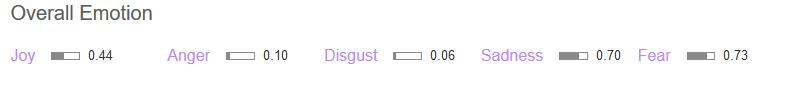
\includegraphics[scale=0.5]{imagens/nlp_sentimentos.jpg}
    \caption{Análise de sentimentos usando IBM Cloud}
    \label{fig:my_label}
\end{figure}{}
\textbf{Análise sintática}: Classifica palavras em classes gramaticais, como substantivos, adjetivos e verbos. \\
\begin{figure}[H]
    \centering
    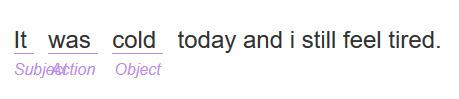
\includegraphics[scale=0.5]{imagens/nlp_analise_sintatica.jpg}
    \caption{Exemplo de análise sintática utilizando IBM Cloud}
    \label{fig:sintatica}
\end{figure}{}
\textbf{Análise de entidades}: Identifica entidades em um texto, como pessoas, locais e produtos. \\
\begin{figure}[H]
    \centering
    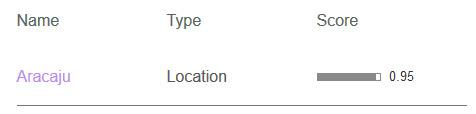
\includegraphics[scale=0.5]{imagens/nlp_entidade.jpg}
    \caption{Exemplo de análise de entidades utilizando IBM Cloud}
    \label{fig:nlp_entidades}
\end{figure}{}
\textbf{Classificação de Conteúdo}: Identifica entidades em um texto e as classifica, a partir de classificações pré-definidas, como pessoas, empresas, lugares, cidades, etc.\\
\begin{figure}[H]
    \centering
    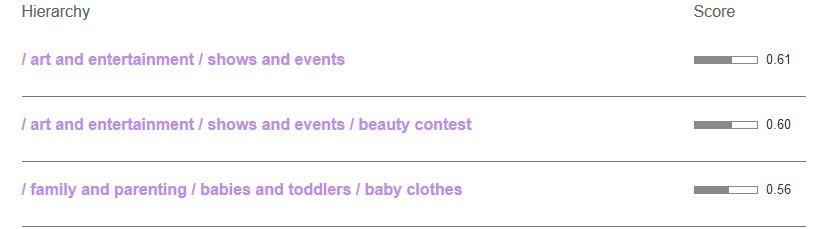
\includegraphics[scale=0.5]{imagens/nlp_classificacao.jpg}
    \caption{Classificação de conteúdo utilizando IBM Cloud}
    \label{fig:nlp_classificacao}
\end{figure}{}
\textbf{Extração de palavras-chave}: Identifica e extrai palavras relevantes em um texto. \\
\begin{figure}[H]
    \centering
    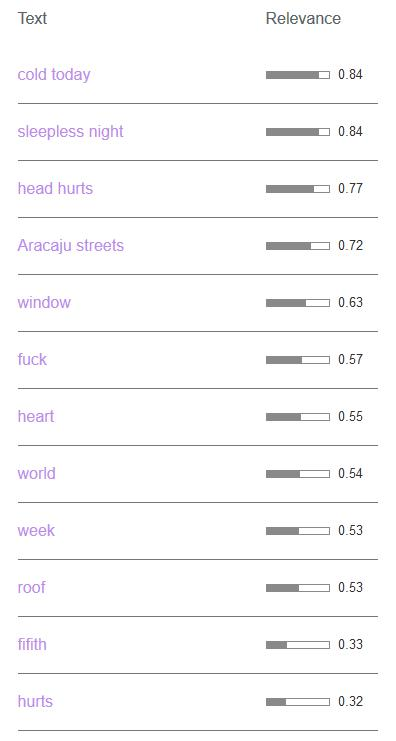
\includegraphics[scale=0.5]{imagens/nlp_extracao_keywords.jpg}
    \caption{Extração de palavras-chave utilizando IBM Cl}
    \label{fig:nlp_keywords}
\end{figure}{}
\textbf{Detecção de idioma}: Identifica o idioma predominante em um texto. \\
\textbf{Text-to-speech}: Ferramentas de sintetização de áudio a partir de textos. \\
\textbf{Speech-to-text}: Ferramentas de transcrição de áudio. \\
\textbf{Chatbot}: Serviços que oferecem uma plataforma, como chats, para tarefas de processamento de linguagem natural. \\
\begin{figure}[H]
    \centering
    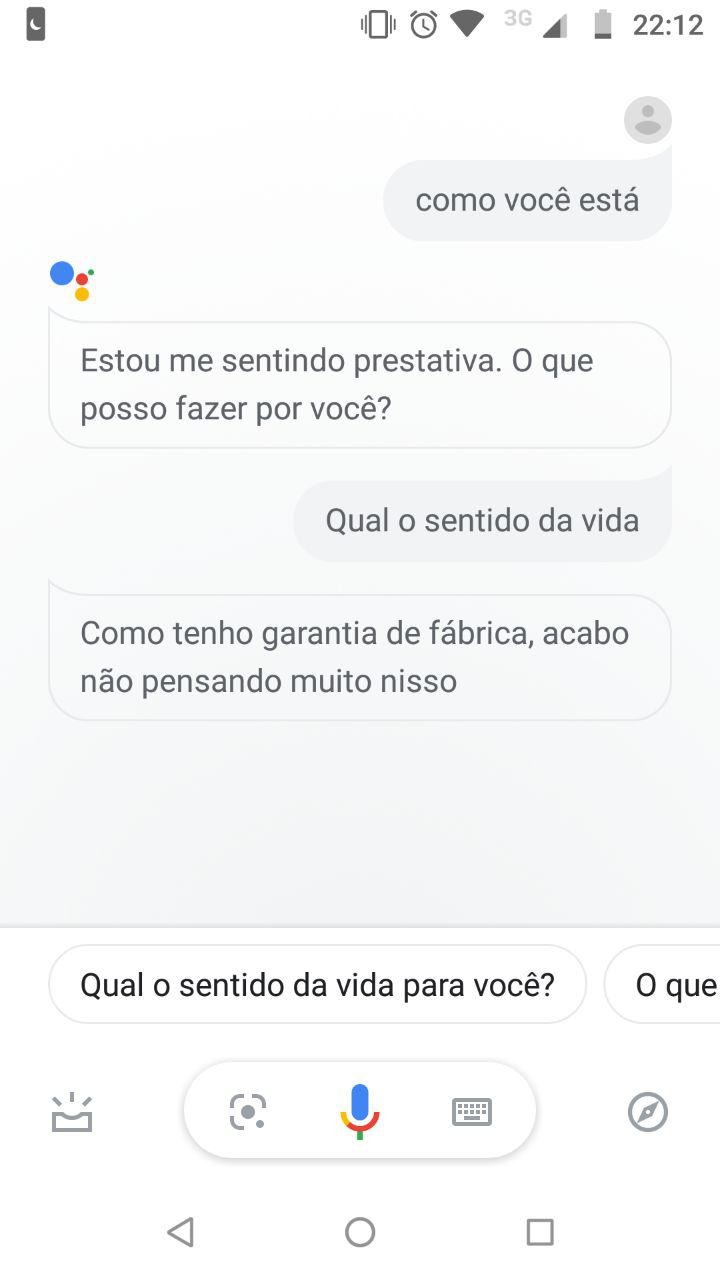
\includegraphics[scale=0.3]{imagens/chatbot.jpg}
    \caption{O Google Assistent é um exemplo de chatbot}
    \label{fig:chatbot}
\end{figure}{}
\textbf{Tradutor}: Ferramentas de tradução, transposição entre idiomas.\\
    \begin{figure}[H]
        \centering
        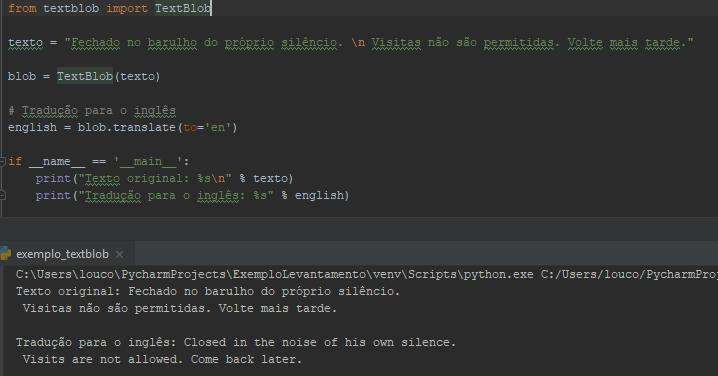
\includegraphics[scale=0.45]{imagens/tradutor.jpg}
        \caption{Exemplo do recurso de tradutor, utilizando TextBlob}
        \label{fig:tradutor}
    \end{figure}
\textbf{Moderador de conteúdo}: Ferramentas que permitem a identificação e censura de palavrões e palavras de baixo calão. \\
\textbf{Reconhecimento do locutor}: Softwares capazes de identificar pessoas através de uma amostra de voz do usuário, o qual precisa ser cadastrado anteriormente. \\

\subsection{Ferramentas de PI}
Nesta subseção, são descritas as 13 tarefas de PI encontradas no levantamento. \\

\textbf{Detecção de categorias em imagens}: Ferramentas para classificar imagens de acordo com categorias pré-definidas, como "praia", "biblioteca", "academia de ginástica", "supermercado", etc.\\
\begin{figure}[H]
    \centering
    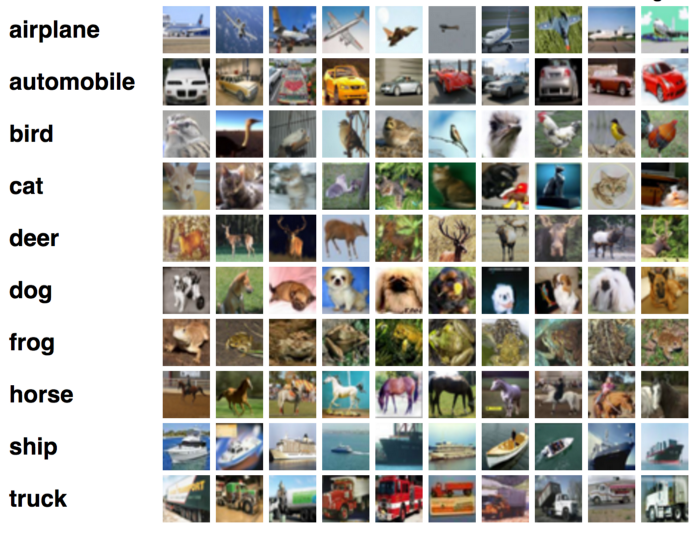
\includegraphics[scale=0.3]{imagens/classificacao_imagens.png}
    \caption{Exemplo de Classificação de Imagens}
    \label{fig:classificação_imagens}
\end{figure}{}
\textbf{Pesquisa por imagens semelhantes}: Tais ferramentas irão buscar por imagens que se assemelham à uma imagem dada como parâmetro. Tais semelhanças podem ser esquemas de cores e objetos presentes na imagem, bem como entidades detectadas. \\
\textbf{Detecção de pontos de referência}: Softwares capazes de reconhecer pontos populares, como Torre Eiffel, Cristo Redentor e outros pontos turísticos ou relevantes como referência.\\
\begin{figure}[H]
    \centering
    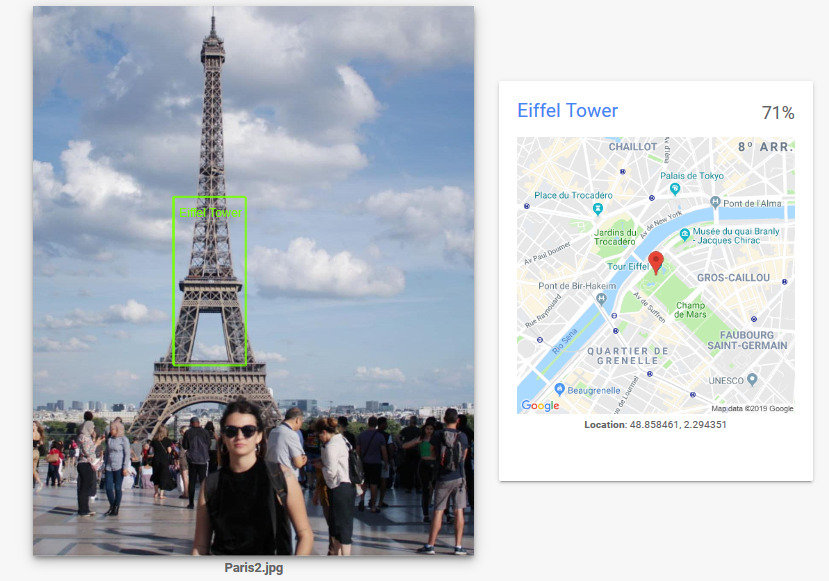
\includegraphics[scale=0.3]{imagens/Paris2.jpg}
    \caption{Detecção de pontos de referência da Google Cloud}
    \label{fig:ponto_turistico}
\end{figure}{}
\textbf{Reconhecimento óptico de caracteres, do inglês: Optical Character Recognition (OCR)}: Softwares capazes de identificar caracteres em uma imagem. A partir dessas ferramentas é possível, por exemplo, transcrever textos através de uma fotografia.\\
\begin{figure}[H]
    \centering
    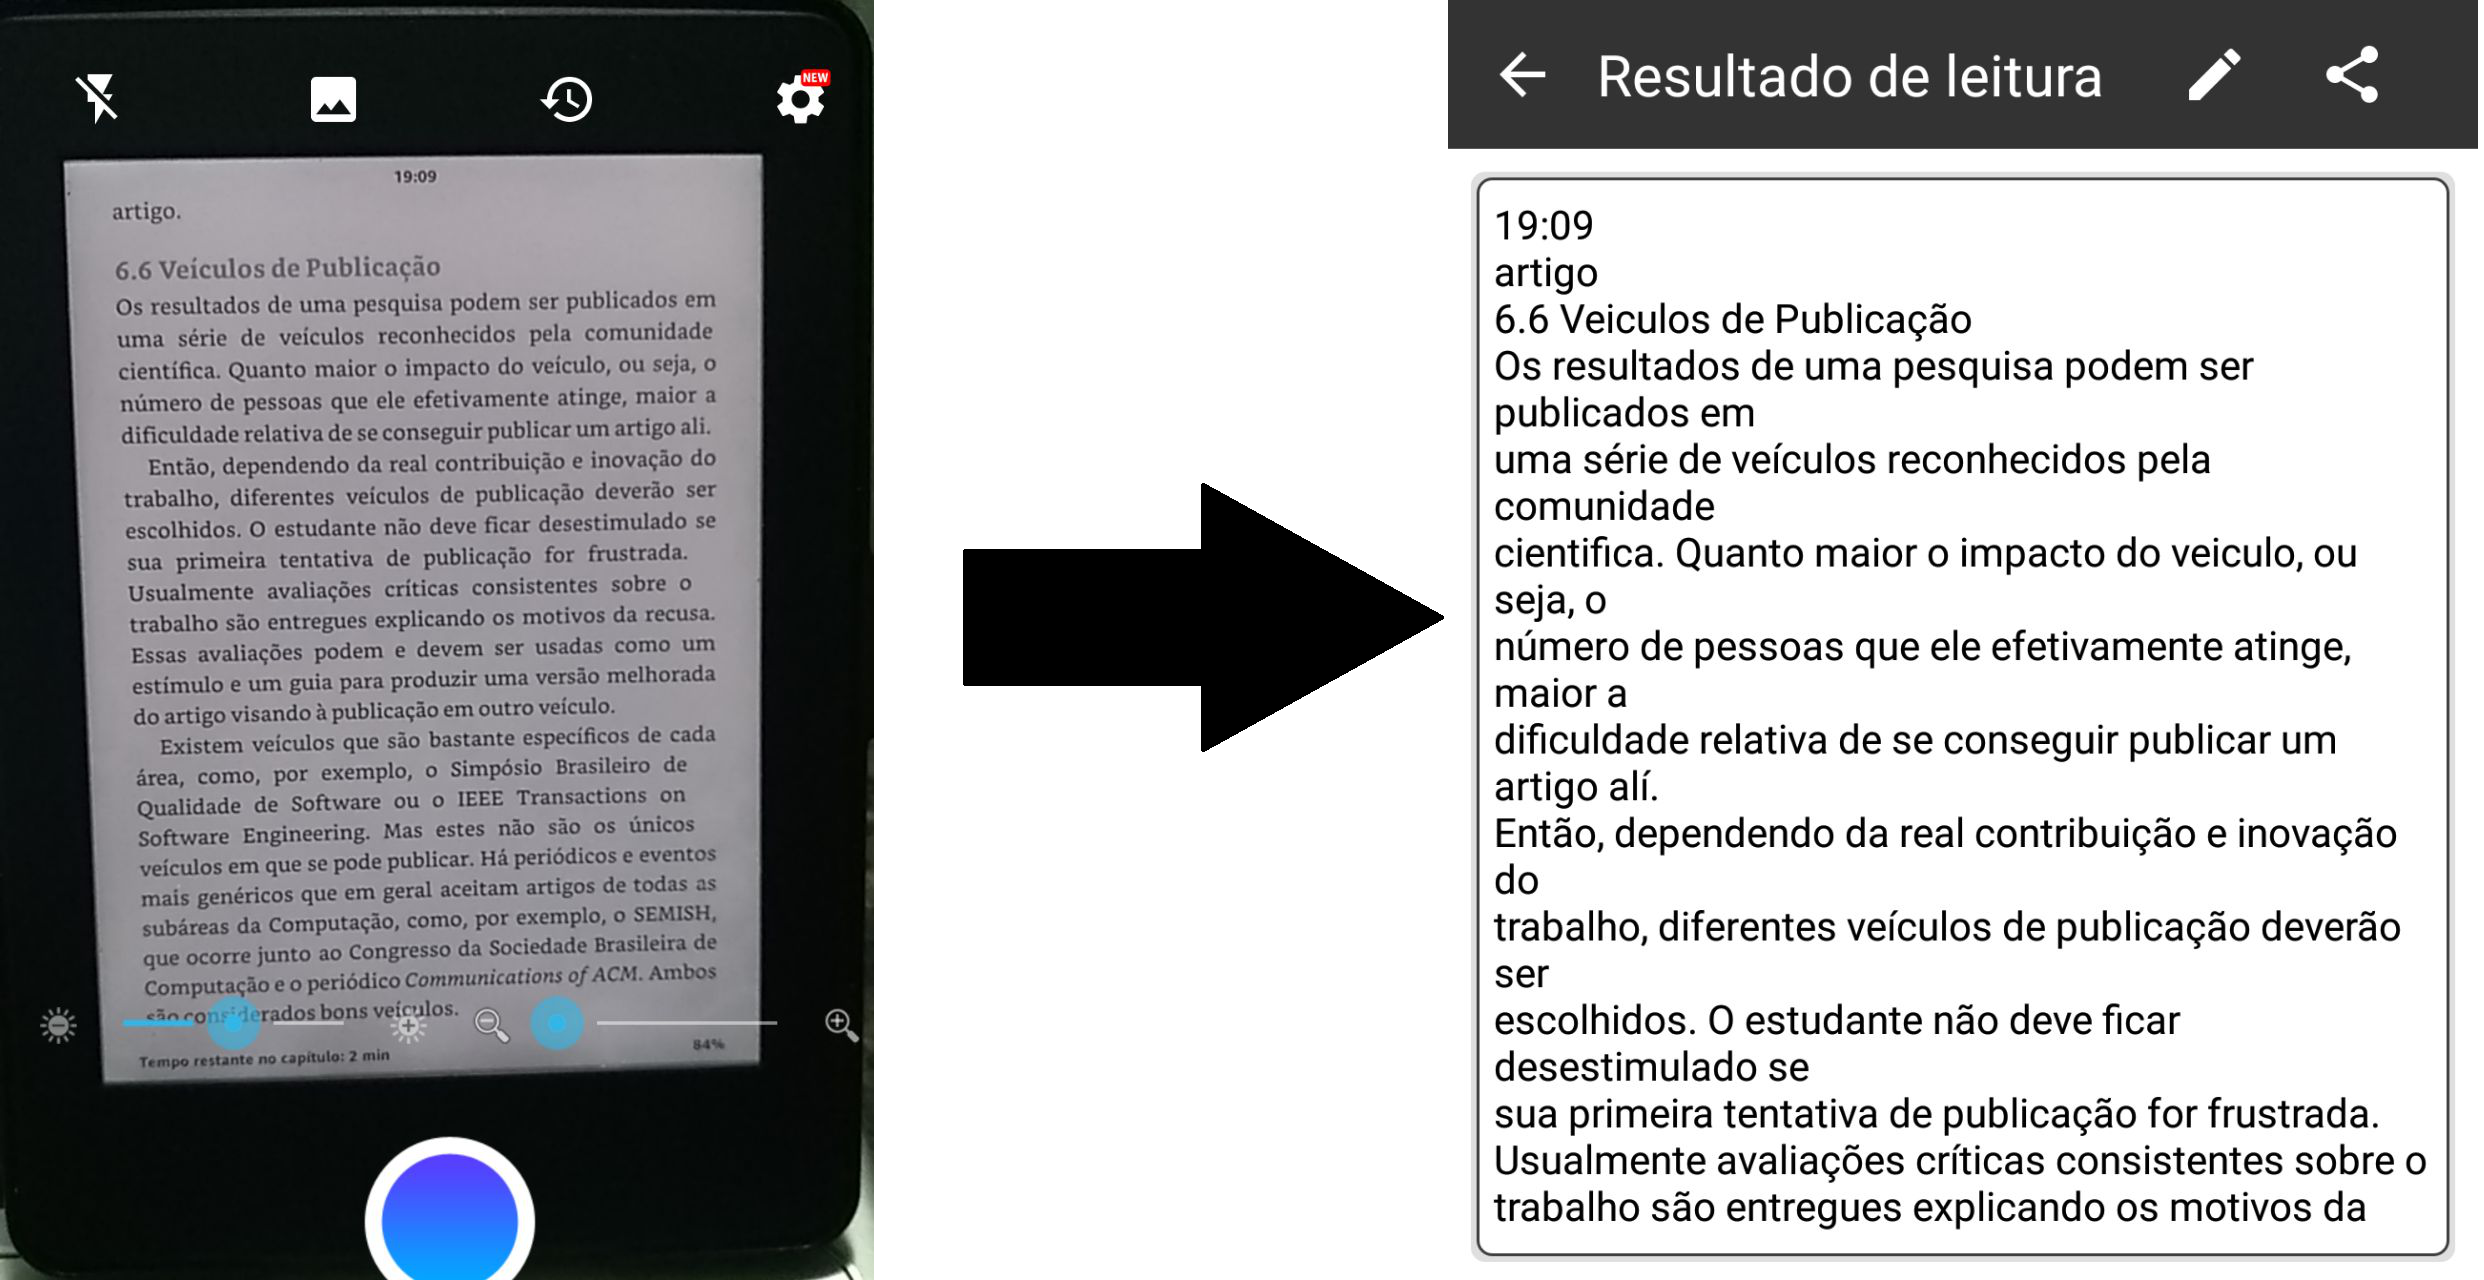
\includegraphics[scale=0.15]{imagens/ocr.png}
    \caption{Exemplo de Reconhecimento óptico de caracteres}
    \label{fig:ocr}
\end{figure}{}
\textbf{Reconhecimento de manuscritos}: Caso particular do reconhecimento óptico de caracteres. Tais ferramentas podem reconhecer, em imagens, textos escritos à mão.\\
% https://towardsdatascience.com/build-a-handwritten-text-recognition-system-using-tensorflow-2326a3487cd5
\begin{figure}[H]
    \centering
    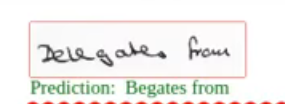
\includegraphics[scale=0.5]{imagens/handwritten.png}
    \caption{Exemplo de reconhecimento de manuscritos}
    \label{fig:manuscrito}
\end{figure}{}
\textbf{Localizador de objetos}: Identifica a posição dos objetos, seus limites retangulares e quantos objetos do mesmo tipo existem na imagem.\\
\begin{figure}[H]
    \centering
    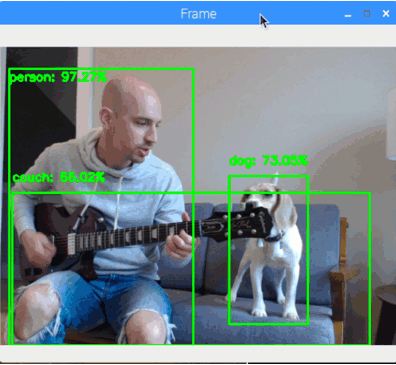
\includegraphics[scale=0.5]{imagens/deteccao_objetos.png}
    \caption{Exemplo da tarefa de detecção de objetos} % https://www.pyimagesearch.com/2019/05/13/object-detection-and-image-classification-with-google-coral-usb-accelerator/
    \label{fig:detecção_obetos}
\end{figure}
\textbf{Detecção facial}: Capacidade de detectar a presença de rostos humanos em imagens, sem necessariamente reconhecer tal rosto.\\
\begin{figure}[H]
    \centering
    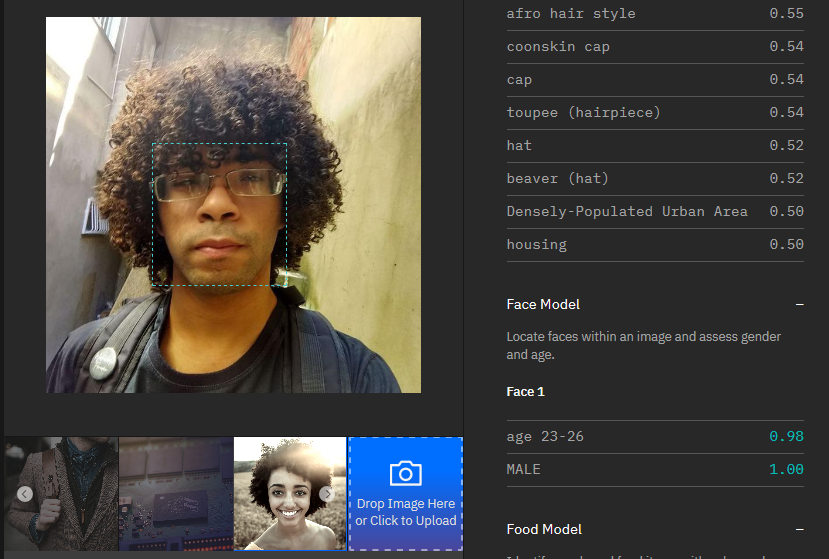
\includegraphics[scale=0.29]{imagens/caracteristicas_watson_visual_recog.png}
    \caption{Exemplo de detecção facial e extração de atributos do IBM Cloud}
    \label{fig:detecção_facial}
\end{figure}{}
\textbf{Moderação de conteúdo}: Softwares para detecção de conteúdo impróprio em imagens, tais como nudez e violência. \\
\textbf{Pesquisa por produtos}: Identifica produtos em uma imagem e busca por produtos semelhantes. \\
\begin{figure}[H]
    \centering
    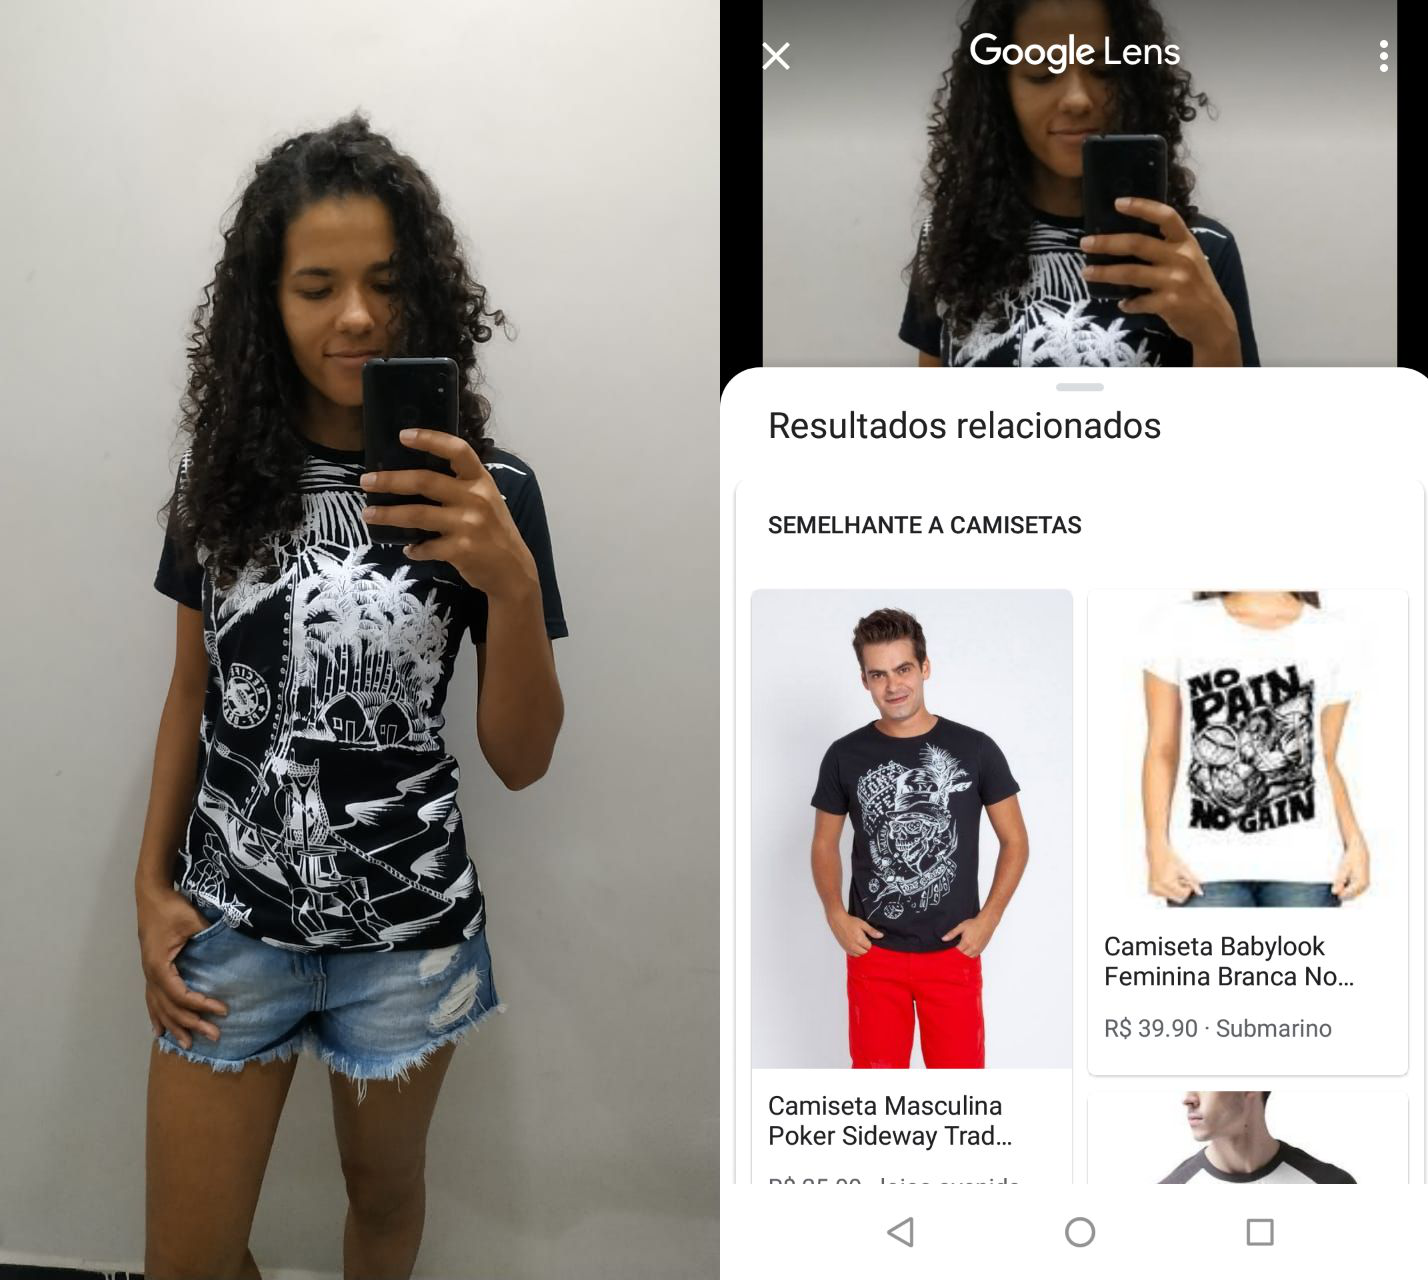
\includegraphics[scale=0.3]{imagens/produtos_semelhantes.png}
    \caption{O Google Lens, para smartphones, possui o recurso de busca por produtos semelhantes}
    \label{fig:produtos_semelhantes}
\end{figure}{}
\textbf{Detecção de atributos}: Identifica atributos como cores dominantes em uma imagem e da sugestões de corte.\\
\begin{figure}[H]
    \centering
    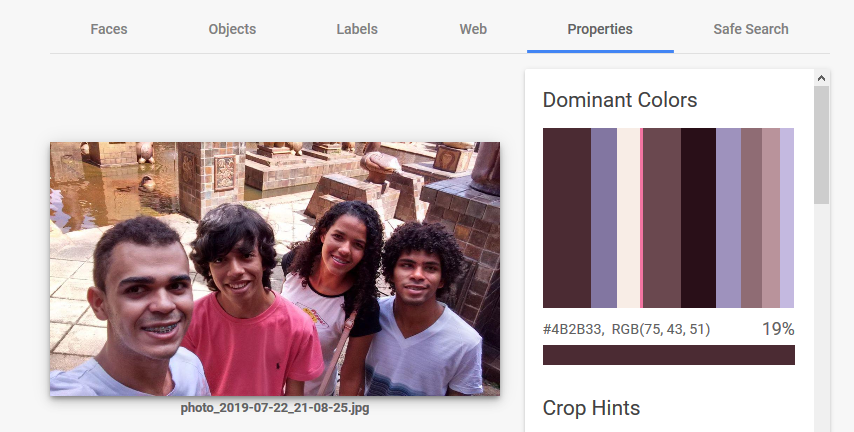
\includegraphics[scale=0.3]{imagens/propriedades.png}
    \caption{Exemplo de detecção de atributos da API Vision do Google Cloud}
    \label{fig:atributos}
\end{figure}{}
\textbf{Reconhecimento facial}: Softwares para reconhecimento de indivíduos em imagens através do seu rosto.\\
\begin{figure}[H]
    \centering
    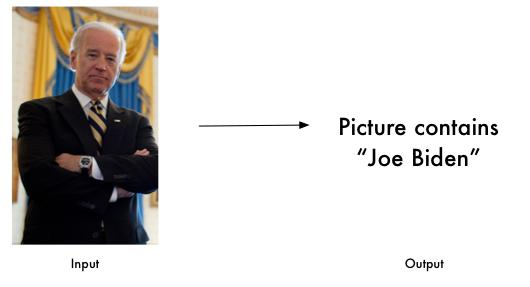
\includegraphics[scale=0.5]{imagens/reconhecimento_facial.jpg}
    % https://github.com/ageitgey/face_recognition
    \caption{Reconhecimento facial}
    \label{fig:reconhecimento_facial}
\end{figure}{}
\textbf{Análise de sentimentos}: Softwares que reconhecem determinados sentimentos, tais quais felicidade, raiva e tristeza através de expressões faciais.\\
\begin{figure}[H]
    \centering
    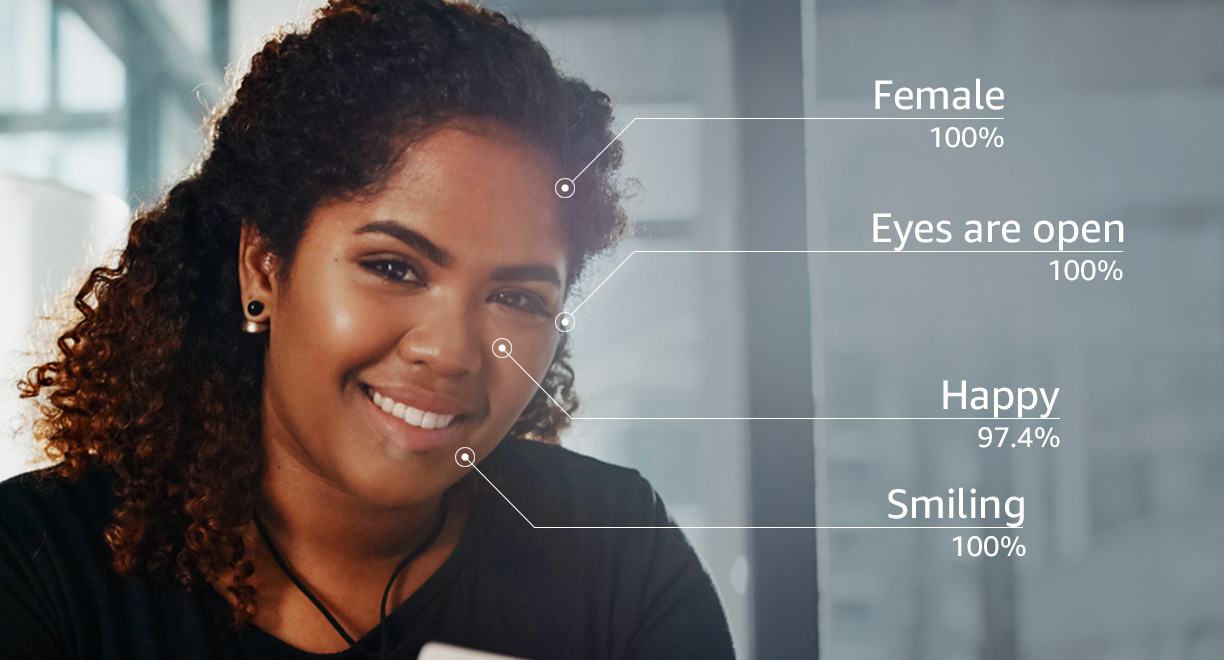
\includegraphics[scale=0.19]{imagens/analise_facial.jpg}
    \caption{Ilustração de análise de sentimentos em imagem da Amazon AWS}
    \label{fig:imagem_sentimentos}
\end{figure}{}
\textbf{Descrição da imagem}: Retorna informações sobre o conteúdo de uma imagem.\\
\begin{figure}[H]
    \centering
    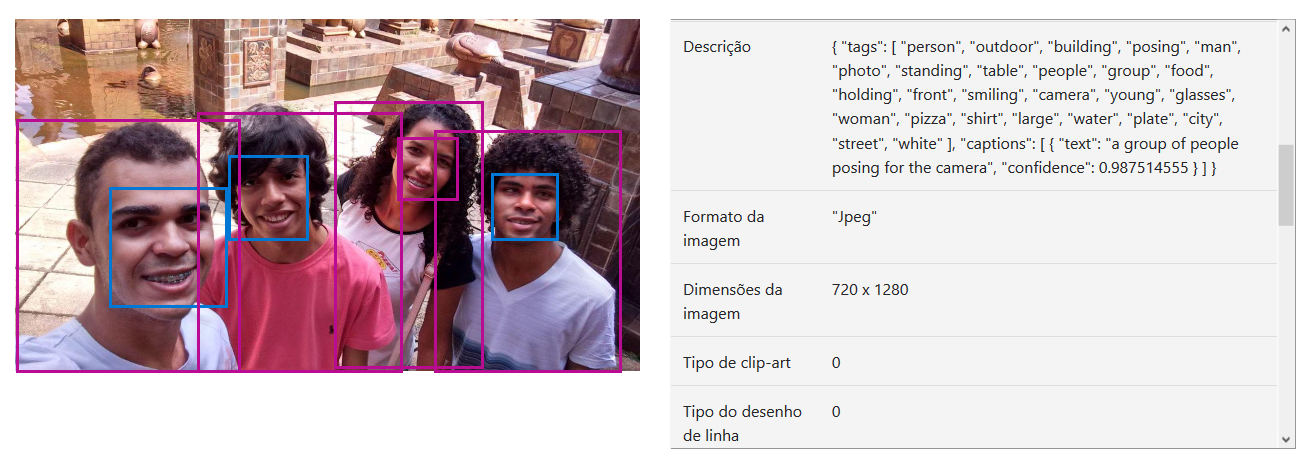
\includegraphics[scale=0.25]{imagens/caption.png}
    \caption{Descrição de imagem da Microsoft Azure}
    \label{fig:captionalize}
\end{figure}{}

\section{Comparativos}

Exibiremos, subsequentemente, tabelas com comparativos entre as ferramentas de cada uma das empresas analisadas. Começamos, na subseção 4.1, comparando a disponibilidade em cada plataforma e em seguida, na subseção 4.2, seus custos.

\subsection{Disponibilidade de ferramentas}
 As tabelas subsequentes ilustram em quais serviços cada tarefa está disponível. Na tabela 1 é exibida a disponibilidade das tarefas de NLP por plataforma e na tabela 2, as de PI. De acordo com a tabela 1, é possível notar que algumas das tarefas encontradas são coincidentes entre as plataformas. Um diferencial sobre o serviço de Text-to-speech da Amazon AWS, o Amazon Polly, é a possibilidade de criar avatares com animações sincronizadas com a fala e destaque de palavras, como em um karaokê. Já o Amazon Textract, a ferramenta de OCR reconhece também o conteúdo de tabelas e formulários. Seu serviço de speech-to-text, o Amazon Transcribe, adiciona pontuação ao texto transcrito, marcações de tempo em relação ao áudio original, personalização de vocabulário, transcrição de streaming e reconhecimento de locutores. Por fim, o Amazon Comprehend, permite o treinamento de modelos de ML através do AutoML\footnote{O serviço AutoML é discutido na subseção 4.2.3}. De forma semelhante ao serviço da Amazon, a IBM Cloud oferece um serviço de speech-to-text em tempo real, capaz de identificar diferentes locutores e customizar o modelo para maior acurácia. Para o serviço de text-to-speech, o principal diferencial do IBM Cloud é a customização das tonalidades de voz e a sintetização para diferentes idiomas. Para o serviço de tradução, também é possível customizar as traduções para terminologias específicas. O serviço de classificação de linguagem da IBM oferece APIs compatíveis com diversas linguagens de programação e um modelo que pode ser treinado pelo usuário para classificações personalizadas. O serviço de speech-to-text da Microsoft também possibilita a identificação dos locutores e a transcrição em tempo real a partir de diversas fontes, como telefones, vídeos e gravações.

\begin{table}[!!ht]
 \caption{Ferramentas de NLP}
  \centering
  \begin{tabular}{lllll}
  \toprule
    \cmidrule(r){1-5}
    Ferramenta & Google Cloud & Amazon AWS & IBM Cloud & Microsoft Azure \\
    \midrule
    Análise de Entidades & X & X & X & X  \\
    Análise de Sentimentos & X & X & X & X   \\
    Análise Sintática & X & X & X & \\
    Classificação de Conteúdo & X & & X & \\
    Extração de palavras-chave & & X & X & X \\
    Text-to-Speech & X & X & X &\\
    Speech-to-Text & X & X & X & X \\
    Chatbot & X & X & & X \\
    Tradutor & X & X & X & X \\
    Moderador de Conteúdo & & & & X \\
    Reconhecimento do Locutor & X & & & \\
    \bottomrule
  \end{tabular}
  \label{tab:table1}
\end{table}

\begin{table}[!!ht]
 \caption{Ferramentas de PI}
  \centering
  \begin{tabular}{lllll}
    \cmidrule(r){1-5}
    Ferramenta & Google Cloud & Amazon AWS & IBM Cloud & Microsoft Azure \\
    \midrule
    Detecção de categorias em imagens & X & X & X & X \\
    Pesquisa por imagens semelhantes & X & & & \\
    Detecção de pontos de referência & X & & & X \\
    OCR & X & X & & X \\
    Reconhecimento de manuscritos & X & & & X \\
    Detecção facial & X & X & X & X \\
    Moderação de conteúdo & X & X & & X \\
    Pesquisa por produtos & X & & & \\
    Detecção de atributos & X & & X & X \\
    Reconhecimento facial & X & X & X & X \\
    Análise de sentimentos & X & X & &  \\
    Descrição da imagem & & & X & X \\
    \bottomrule
  \end{tabular}
  \label{tab:table2}
\end{table}

\subsection{Comparativo de preços}

Nesta seção, comparamos os preços das ferramentas analisadas entre as empresas que oferecem tais serviços. Na subseção 4.2.1, são comparados os preços entre as ferramentas de NLP e na subseção 4.2.2, as ferramentas de PI.

\subsubsection{Ferramentas de NLP}

Nas tabelas subsequentes, são exibidos os comparativos de preços por ferramenta, quando há coincidência de disponibilidade. Em primeiro caso, comparamos os serviços de NLP. Análise de sentimentos, reconhecimento de entidades, análise sintática, text-to-speech, speech-to-text e extração de palavras-chave. Na tabela 3, comparamos a disponibilidade gratuita desses serviços e na tabela 4, comparamos seus custos.

\begin{table}[!!ht]
 \caption{Disponibilidade gratuita dos serviços básicos de NLP}
  \centering
  \begin{tabular}{lllll}
    \cmidrule(r){1-5}
    Serviço & Google Cloud & Amazon AWS & IBM Cloud & Microsoft Azure \\
    \midrule
    Análise de sentimentos & \makecell{Até 5k unidades} & \makecell{5M de caracteres mensais \\ durante 12 meses} & \makecell{30k de caracteres \\ por mês} & \makecell{5k transações por mês} \\
    Reconhecimento de entidades & \makecell{Até 5k unidades} & \makecell{Integrado} & \makecell{Integrado} & \makecell{Integrado} \\
    Análise sintática & \makecell{Até 5k unidades} & \makecell{Integrado} & \makecell{Integrado} & \makecell{N/A} \\
    Extração de palavras-chave & \makecell{N/A} & \makecell{Integrado} & \makecell{Integrado} & \makecell{Intrgrado} \\
    \bottomrule
  \end{tabular}
  \label{tab:table3}
\end{table}

\begin{table}[!!ht]
 \caption{Comparativo dos serviços de NLP, na faixa 10 milhões a 50 milhões de unidades}
  \centering
  \begin{tabular}{lllll}
    \cmidrule(r){1-5}
    Serviço & Google Cloud & Amazon AWS & IBM Cloud & Microsoft Azure \\
    \midrule
    Análise de sentimentos & \makecell{US\$ 0,50}  & \makecell{US\$ 0,00005} & \makecell{US\$ 0,001} & \makecell{US\$ 0,25} \\
    Reconhecimento de entidades & \makecell{ US\$ 0,50} & \makecell{US\$ 0,00005} & \makecell{US\$ 0,001} & \makecell{US\$ 0,25} \\
    Análise sintática & \makecell{US\$ 0,25} & \makecell{US\$ 0,0000025} & \makecell{US\$ 0,001} & \\
    Text-to-speech & \makecell{US\$ 4 / 1M \\ de caracteres} & \makecell{US\$ 4 / 1M \\ de caracteres} & \makecell{US\$ 0,02 / \\ 1M de caracteres} & \\
    Speech-to-text & \makecell{US\$ 0,006} & \makecell{US\$ 0,006} & \makecell{US\$ 0,01} & \makecell{US\$ 0,04} \\
    Extração de palavras-chave & & \makecell{US\$ 0,00005} & \makecell{US\$ 0,001} & \makecell{US\$ 0,25} \\
    \bottomrule
  \end{tabular}
  \label{tab:table4}
\end{table}

Na Google Cloud, o serviço de Classificação de Conteúdo é cobrado pela chamada de API por unidade. Uma unidade é considerada, levando em conta tags HTML, XML, espaços, etc. Os valores no Google Cloud são cobrados de acordo com a quantidade de chamadas da API por mês. No caso do IBM Cloud, o usuário é cobrado separadamente por chamada da API, por classificador e por evento de treinamento. Ambos oferecem um mínimo grátis mensal, detalhado na tabela 4.

\begin{table}[!!ht]
 \caption{Comparativo entre a taxa de serviços grátis de Classificação de Conteúdo do Google Cloud e do IBM Cloud}
  \centering
  \begin{tabular}{lll}
    \cmidrule(r){1-3}
    Serviço & Google Cloud & IBM Cloud \\
    \midrule
    Classificador & até 30.000 unidades por mês  & 1 classificador grátis por mês \\
    Chamadas de API & & 1000 chamadas por mês \\
    Eventos de treinamento & & 4 eventos por mês \\
    \bottomrule
  \end{tabular}
  \label{tab:table5}
\end{table}

\begin{table}[!!ht]
 \caption{Comparativo do serviço de Classificação de Conteúdo entre Google Cloud e IBM Cloud}
  \centering
  \begin{tabular}{lll}
    \cmidrule(r){1-3}
    Serviço & Google Cloud & IBM Cloud \\
    \midrule
    Classificação de Conteúdo & US\$ 0,10 / mês, para mais de 5M de unidades & US\$0.0035 / chamada de API \\
    \bottomrule
  \end{tabular}
  \label{tab:table6}
\end{table}

Serviços de tradução foram encontrados em todas as plataformas. A Google Cloud oferece dois serviços de tradução: uma API com um modelo de ML pré-treinado e a AutoML Translation, que permite o treino de um modelo de ML para serviços de tradução. A IBM Cloud oferece quatro tipos de planos para seu serviço de tradução: Lite, Standard, Advanced e Premium. Para fins de comparação, levaremos em conta o plano lite. A Microsoft Azure, ao contrário dos anteriores, oferece serviço de tradução apenas para fala em dois contêiners: um grátis, que permite apenas uma solicitação e o contêiner padrão, que permite até 20 solicitações simultaneamente. Todos os serviços, exceto Google Cloud, contam com detecção automática do idioma integrada.

\begin{table}[!!ht]
 \caption{Disponibilidade gratuita dos serviços de Tradutor}
  \centering
  \begin{tabular}{lllll}
    \cmidrule(r){1-5}
    Serviço & Google Cloud & Amazon AWS & IBM Cloud & Microsoft Azure \\
    \midrule
    Tradução de textos & \makecell{Até 5k caracteres} & \makecell{2M de caracteres mensais \\ durante 12 meses} & \makecell{1M de caracteres \\ por mês} & \makecell{2M de caracteres \\ por mês}  \\
    \bottomrule
  \end{tabular}
  \label{tab:table7}
\end{table}

\begin{table}[!!ht]
 \caption{Comparativo do serviço de Tradutor entre Google Cloud, Amazon AWS, IBM Cloud e Microsoft Azure (por 1M de caracteres mensais}
  \centering
  \begin{tabular}{lllll}
    \cmidrule(r){1-5}
    Serviço & Google Cloud & Amazon AWS & IBM Cloud & Microsoft Azure \\
    \midrule
    Tradução de textos & \makecell{US\$ 20} & \makecell{US\$ 15} & Gratuito\footnote{Acima dos primeiros 250k caracteres, é cobrada uma taxa de US\$ 0,02 por 1k de caracteres.} & \makecell{US\$ 9,89}  \\
    AutoML & \makecell{US\$ 76 por \\ hora de treinamento} & & \\
    Detecção de idiomas & \makecell{US\$ 20} & & US\$ 0,25 \\
    Tradução de fala & & & & \makecell{5 horas gratuitas mensais \\ de áudio (contêiner grátis)} \footnote{ou US\$ 2,43 / hora de áudio (contêiner padrão)} \\
    AutoML (predição) & Gratuito (até 5M caracteres) \footnote{ou US\$ 80 por milhão de caractere} & & & \\
    \bottomrule
  \end{tabular}
  \label{tab:table8}
\end{table}

Todas as empresas analisadas oferecem o serviço de speech-to-text. Nas tabelas 7 e 8, são comparados os planos gratuitos e pagos, respectivamente. Uma ressalva quanto ao serviço gratuito da Microsoft Azure é que este oferece 4 recursos: Padrão, fala personalizada, hospedagem do ponto de extremidade da fala personalizada e áudio multicanal de transcrição de conversas. Exceto pela hospedagem, que oferece apenas um modelo gratuito por mês, são disponibilizados 5 horas de áudio por mês para cada recurso.
A Google Cloud oferece o serviço de speech-to-text em quatro formatos. Primeiramente, temos o modelo padrão, sem smartphone e vídeo aprimorados com dois recursos: reconhecimento de fala sem geração de registro de dados e com geração de registro. Já no modelo Premium, são oferecidos os mesmos recursos com smartphone e vídeo aprimorados. Para construção da tabela consideramos o modelo Premium com geração de registro de dados.

\begin{table}[!!ht]
 \caption{Comparativo do serviço de Speech-to-text gratuitos}
  \centering
  \begin{tabular}{lllll}
    \cmidrule(r){1-5}
    Serviço & Google Cloud & Amazon AWS & IBM Cloud & Microsoft Azure \\
    \midrule
    Speech-to-text & até 60 minutos & até 60 minutos / mês durante 12 messes & 500 minutos / mês & 300 minutos / mês \\
    \bottomrule
  \end{tabular}
  \label{tab:table9}
\end{table}

Um detalhe sobre os serviços de Speech-to-text, é que a Amazon AWS o usuário é cobrado em US\$ 0,0004 por segundo mais o acréscimo mínimo de US\$ 0,006 pelos 15 primeiros segundos. O IBM Cloud possui também o plano Premium, o qual não tem os preços acessíveis no site, para esse plano, os preços devem ser combinados com a empresa. Para o serviço da Microsoft azure, consideramos o plano padrão na tabela comparativa, os demais são exibidos na tabela 8.

\begin{table}[!!ht]
 \caption{Preços dos demais serviços de speech-to-text da Microsoft Azure (por hora)}
  \centering
  \begin{tabular}{ll}
    \cmidrule(r){1-2}
    Serviço & Preço \\
    \midrule
    Fala personalizada & US\$ 1,39\\ % R\$ 5,201
    Hospedagem do ponto de extremidade da fala personalizada & US\$ 39,59 \\ % R\$ 148,6
    Áudio multicanal de transcrição de conversas & Não Disponível \\
    \bottomrule
  \end{tabular}
  \label{tab:table10}
\end{table}

Todas as empresas analisadas oferecem serviços para a construção de chatbots. Na Google Cloud, temos o DialogFlow que utiliza ML para customizar os tipos de entidade que podem ser reconhecidas pelo chatbot a partir de um conjunto de dados inicial fornecido pelo usuário desenvolvedor. O DialogFlow também faz uso das APIs de text-to-speech e speech-to-text para criar bots que se comunicam por voz com o usuário final. Através do serviço de Analytics da Google, o chatbot pode ser otimizado para atender os interesses da sua organização. Além disso, o bot conta também com análise de sentimentos, para melhor atender ao usuário final. O serviço da Amazon, o AWS Lex, utiliza a mesma tecnologia utilizada na Alexa para construir bots com análise de sentimentos, compreensão de fala e escrita. O AWS Lex também oferece fácil integração com outros serviços da Amazon AWS, como lógica de negócios, banco de dados, segurança, desenvolvimento de aplicativos móveis. etc. O Watson Assistent, da IBM, possui o recurso de direcionar o usuário para plataformas como Slack e Facebook Messenger, além de direcionar o usuário para um atendente humano quando necessário. Através do sistema de digressões, o chatbot feito a partir do IBM Watson pode ir de um tópico a outro em uma conversa e retornar ao primeiro tópico posteriormente. O chatbot também pede para o usuário ser mais claro quando é feito um pedido ambíguo ou incompreensível, evitando respostas erradas. Por fim, o serviço de bot do Azure também permite integração com canais de comunicação, como Slack e Facebook Messenger. Como os serviços anteriores, também possui suporte, tanto para a interação por texto, quanto por fala. Além disso, também é possível interagir através de imagens em anexo; o Azure utilizará seus próprios serviços de PI para interagir com imagens em anexo enviadas pelo usuário final. Nas tabelas 9 e 10, fazemos comparativos entre os serviços gratuitos e pagos, respectivamente. 
O plano padrão da Google Cloud, citado na tabela 9, compreende os recursos de texto e entrada e saída de áudio.

\begin{table}[!!ht]
 \caption{Disponibilidade gratuita dos serviços de chatbot}
  \centering
  \begin{tabular}{llll}
    \cmidrule(r){1-4}
    Google Cloud & Amazon AWS & IBM Cloud & Microsoft Azure \\
    \midrule
    Plano padrão gratuito
    & \makecell{10k solicitações de texto e \\ 5k solicitações de fala\footnote{Durante o período gratuito de 12 meses}}
    & 30 dias gratuitos
    & \makecell{Mensagens ilimitadas em canais Standard\\ e 1k de mensagens por mês em Canais Premium\footnote{Canais Premium são os serviços da Microsoft, como o Skype e canais populares, como o Facebook Messenger. Canais Premium são a aplicação personalizada do usuário desenvolvedor}} \\
    \bottomrule
  \end{tabular}
  \label{tab:table11}
\end{table}

\begin{table}[!!ht]
 \caption{Preços dos serviços de chatbot (por solicitação)}
  \centering
  \begin{tabular}{lllll}
    \cmidrule(r){1-5}
    Serviço & Google Cloud & Amazon AWS & IBM Cloud & Microsoft Azure \\
    \midrule
    Texto & \makecell{US\$ 0,002} & \makecell{US\$ 0,00075} & \makecell{US\$0.0025 \\ por mensagem} & \makecell{US\$ 0,0005} \\
    Entrada de áudio & \makecell{US\$ 0.0065 por \\  15 segundos de áudio } & \makecell{US\$0,0065 por \\ 15 segundos de áudio}  & & \makecell{Integrado}\\
    Saída de áudio & \makecell{US\$ 4 por 1M de \\ caracteres (Vozes padrão)} & \makecell{Integrado} & & \makecell{Integrado} \\
    Análise de sentimentos & \makecell{US\$ 0,25 para cada \\ 1k de solicitações, entre 5M e \\ 20M de solicitações} & \makecell{Integrado} & & \makecell{Integrado}\\
    \bottomrule
  \end{tabular}
  \label{tab:table12}
\end{table}

\subsubsection{Processamento de Imagem}

Para o serviço de PI, a Amazon oferece a API Rekognition que, além de analisar imagens, permite também a análise de vídeos. Além disso, o serviço conta com aprimoramento contínuo através de algoritmos de ML. De forma semelhante, a IBM Cloud também permite treinar modelos para criar classificadores. A Google Cloud oferece uma API REST para as tarefas de PI, a API Cloud Vision, que utiliza modelos pré treinados e  o Auto ML (Beta) para treinar modelos de ML. Além disso, há também a Cloud Video Intelligence, para extrair metadados de vídeos. Os planos gratuitos de PI são comparados na tabela 11 e os planos pagos, na faixa de 5M de unidades, na tabela 12.

\begin{table}[!!ht]
 \caption{Disponibilidade gratuita dos serviços}
  \centering
  \begin{tabular}{llll}
    \cmidrule(r){1-4}
    Google Cloud & Amazon AWS & IBM Cloud & Microsoft Azure \\
    \midrule
    1k de unidades & 5k de unidades durante 12 meses & 250MB de memória Cloud Foundry & 5k de transações por mês \\
    \bottomrule
  \end{tabular}
  \label{tab:table13}
\end{table}

\begin{table}[!!ht]
 \caption{Comparativo dos serviços de PI (até 5M de caracteres mensais)}
  \centering
  \begin{tabular}{lllll}
    \cmidrule(r){1-5}
    Serviço & Google Cloud & Amazon AWS & IBM Cloud & Microsoft Azure \\
    \midrule
    Detecção de categorias em imagens & US\$ 1,50 & US\$ 0,8 & US\$ 0,0011 & US\$ 0,79 \\ %R\$0,00431
    Detecção de pontos de referência & US\$ 1,50 & & & US\$ 0,64 \\
    OCR & US\$ 1,50 & US\$ 0,0006 / página & & US\$ 0,64 por cada 1k de transações \\ % R\$ 2,415
    Reconhecimento de manuscritos & US\$ 1,50 & & & US\$ 2,47 por cada 1k de transações \\ % R\$ 9,287
    Localizador de objetos & US\$ 2,25 & & & US\$ 0,79 \\
    Detecção facial & US\$ 1,50 & & US\$ 0,0023 & US\$ 0,59 por cada 1k de transações \\ % R\$ 0,008639 & R\$ 2,229
    Moderação de conteúdo & US\$ 1,50 \footnote{gratuito se comprado junto com Detecção de categorias}& US\$ 0,8 & & US\$ 0,59 por cada 1k de transações \\
    Detecção de atributos & US\$ 1,50 & & & US\$ 0,79 \\
    Reconhecimento facial & US\$ 1,50 & US\$ 0,8 & US\$ 0,0011 & US\$ 0,59 por cada 1k de transações \\ % R\$ 0,004039
    Análise de sentimentos & US\$ 1,50 & US\$ 0,8 & & \\
    Descrição da imagem & & & & US\$ 2,47 \\
    \bottomrule
  \end{tabular}
  \label{tab:table14}
\end{table}

\subsubsection{Treinamento de modelos de aprendizado de máquina}
Traremos destaque, nesta subseção, para os serviços que permitem o treinamento de modelos de ML, integrados ou não. Na tabela 13, tabelamos essa informação tanto dos serviços de NLP quando dos serviços de PI.

Iniciando pela Google Cloud, temos o serviço de PI, o Auto ML Vision (Beta). A partir dele, é possível treinar classificadores e marcar pessoas com ou sem rótulos predefinidos. Esse serviço é gratuito para até 1k de imagens previstas por mês e para uma hora de treinamento. Para a análise de vídeos, há a API Video Intelligence, que possui uma interface gráfica e uma API REST, e permite classificar vídeos a partir de rótulos personalizados e detecta mudanças no cenário de um vídeo. Para as tarefas de NLP, a Google Cloud disponibiliza a AutoML Natural Language (Beta) e a AutoML Translation (Beta). O primeiro permite a criação e a classificação de entidades, sentimentos e outros modelos personalizados. Já o segundo permite o treinamento de modelos de ML para obter traduções mais fiéis e adaptadas a determinados contextos. Para a Amazon AWS, não foram encontrados serviços de treinamento para modelos de ML voltados a programadores sem conhecimento técnico. Na Amazon AWS, o único serviço que oferece personalização por modelos de ML, é o Amazon Comprehend.\footnote{Supracitado na subseção 4.1}
O serviço de tradução da IBM Cloud oferece um serviço de customização, baseado em ML. Para tal serviço, é cobrada uma taxa de US\$ 0,10 para cada 1k de caracteres. O serviço de classificação de linguagem natural da IBM também possibilita o treinamento de modelos, para os quais são oferecidos 4 treinamentos gratuitos por mês. Na Microsoft Azure, é possível treinar modelos para transcrição personalizada em seu serviço de speech-to-text.

\section{Aplicação}

\section{Conclusão}
\label{sec:headings}


% \bibliographystyle{unsrt}  
%\bibliography{references}  %%% Remove comment to use the external .bib file (using bibtex).
%%% and comment out the ``thebibliography'' section.


%%% Comment out this section when you \bibliography{references} is enabled.
% \begin{thebibliography}{1}
% George Kour and Raid Saabne.
% \newblock Real-time segmentation of on-line handwritten arabic script.
% \newblock In {\em Frontiers in Handwriting Recognition (ICFHR), 2014 14th
% International Conference on}, pages 417--422. IEEE, 2014.

% \bibitem{kour2014fast}
% George Kour and Raid Saabne.
% \newblock Fast classification of handwritten on-line arabic characters.
% \newblock In {\em Soft Computing and Pattern Recognition (SoCPaR), 2014 6th
%   International Conference of}, pages 312--318. IEEE, 2014.

% \bibitem{hadash2018estimate}
% Guy Hadash, Einat Kermany, Boaz Carmeli, Ofer Lavi, George Kour, and Alon
%  Jacovi.
% \newblock Estimate and replace: A novel approach to integrating deep neural
%  networks with existing applications.
% \newblock {\em arXiv preprint arXiv:1804.09028}, 2018.

%\end{thebibliography}


\end{document}
